\begin{figure}[ht]
    \centering
    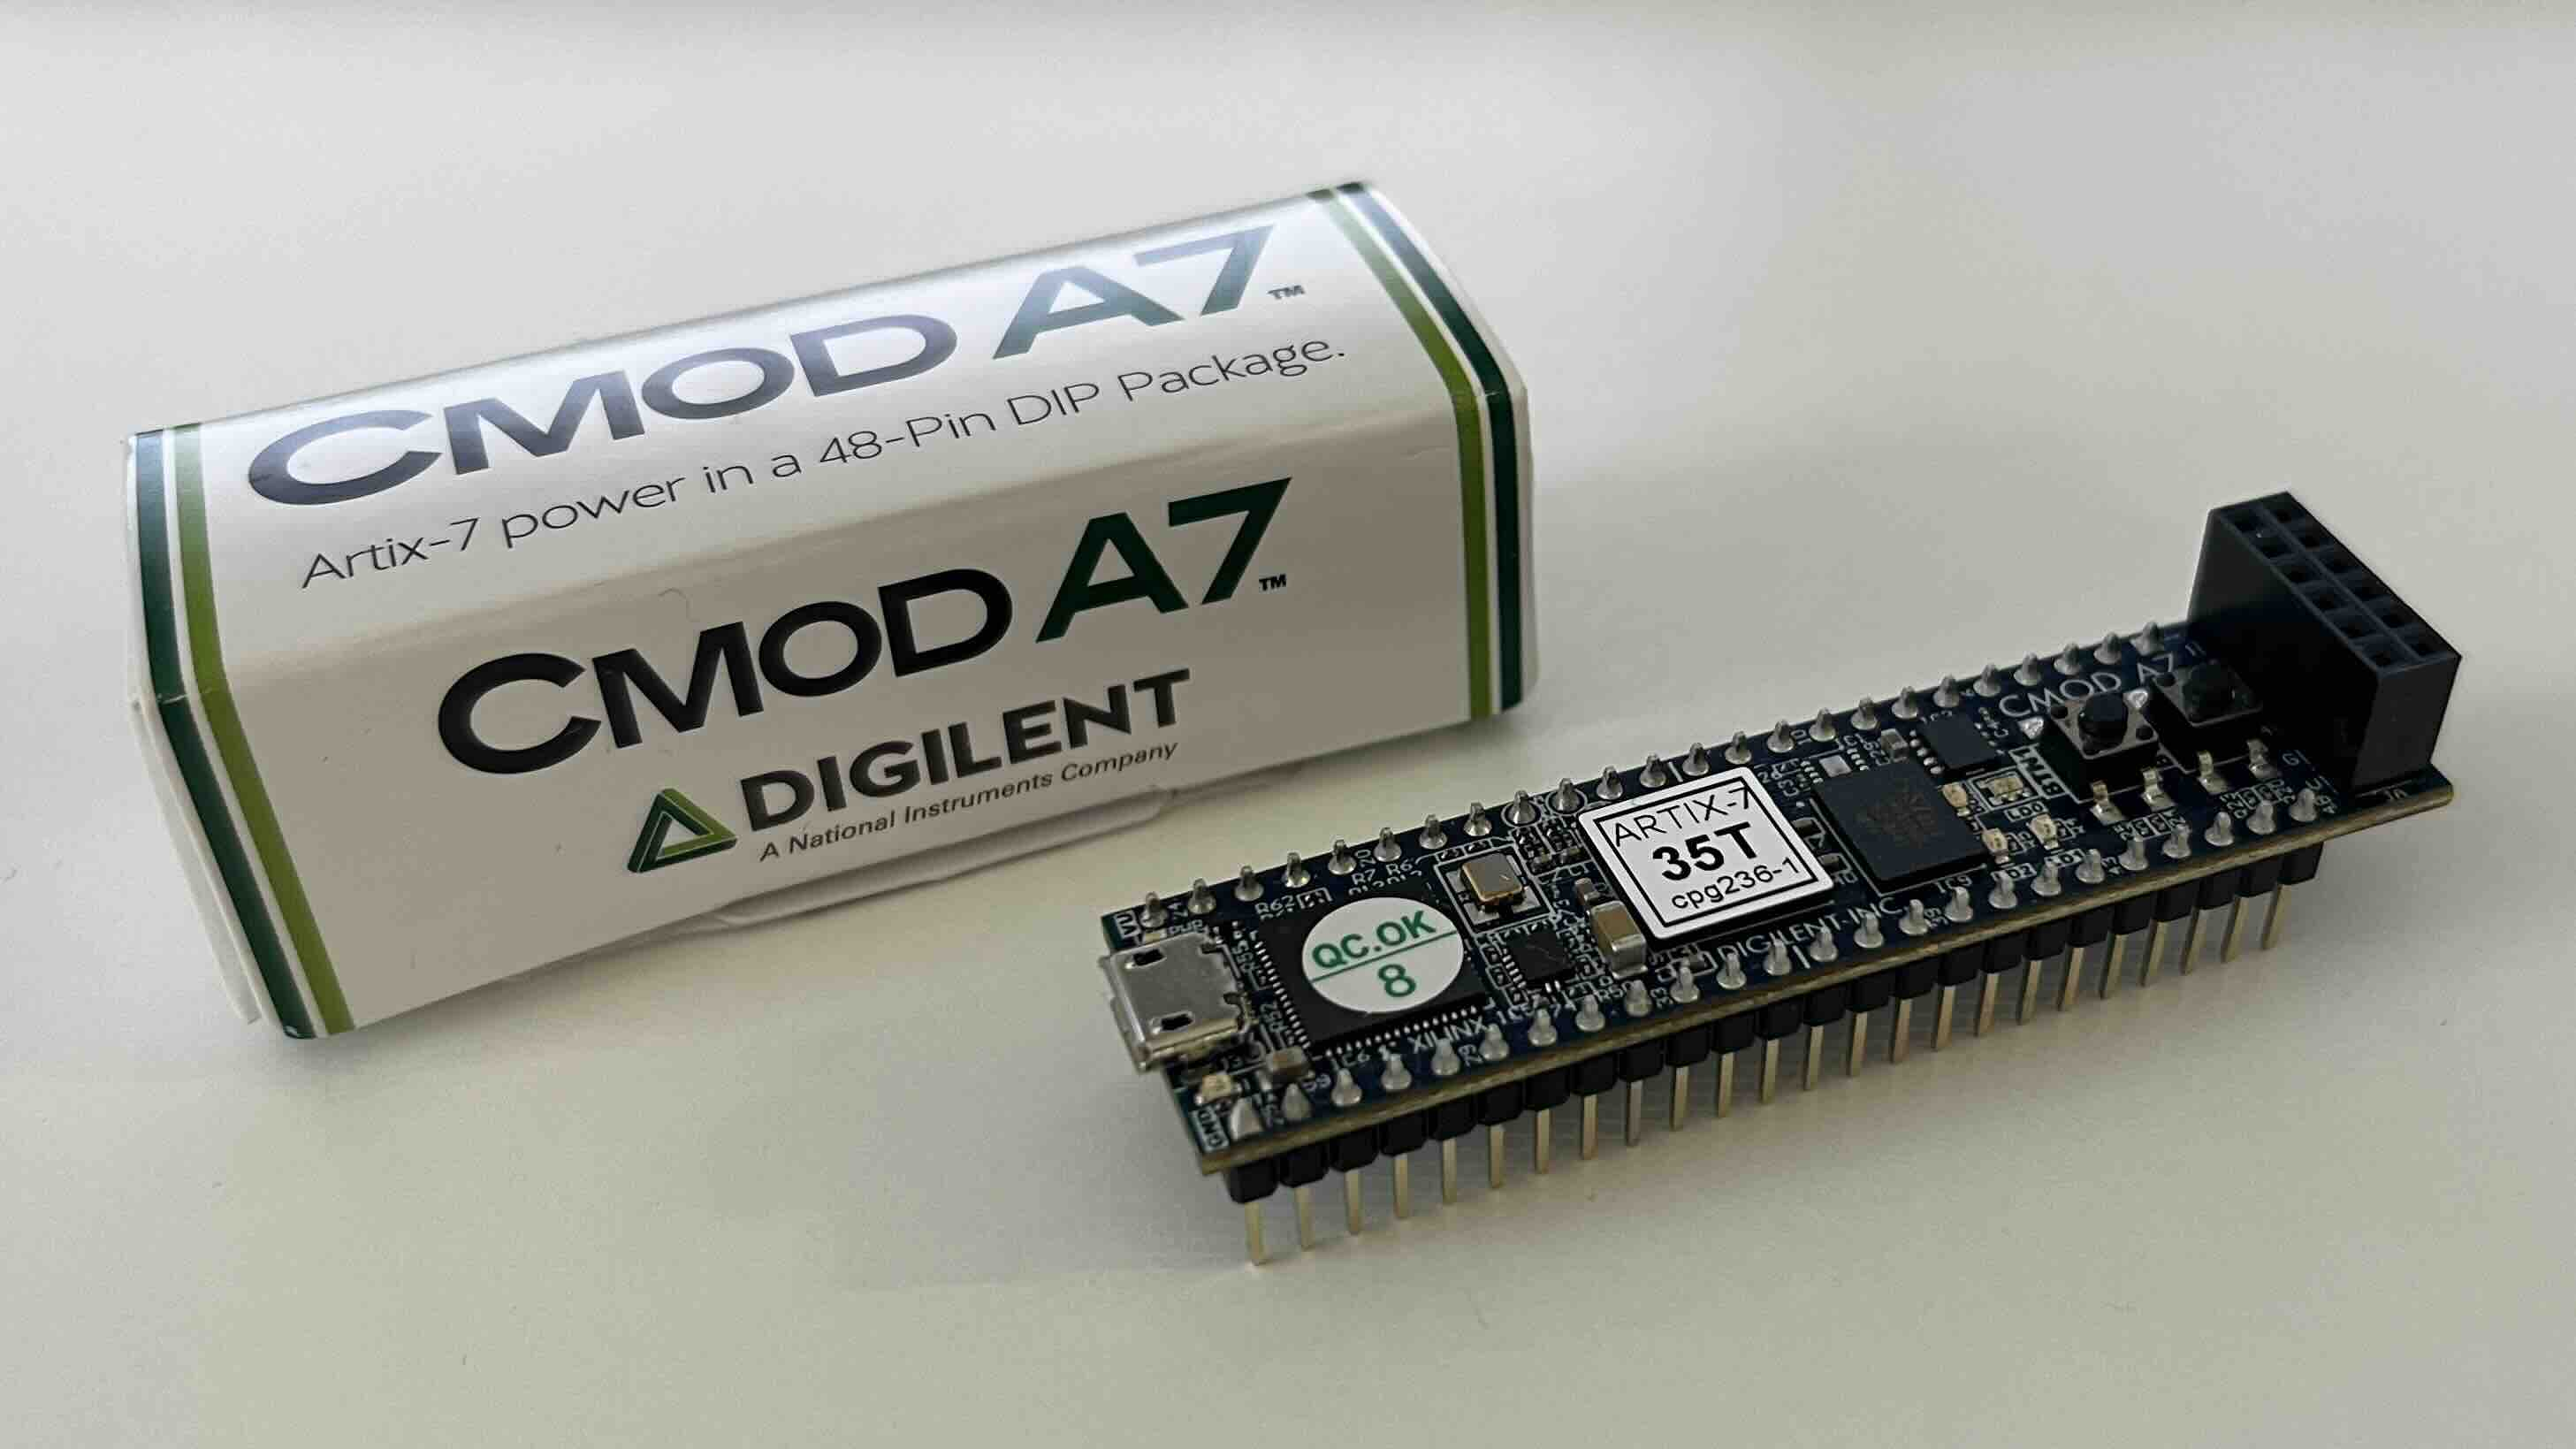
\includegraphics[width=0.5\columnwidth]{images/chapter_2/digilent.jpeg}
    \caption{The Digilent Cmod A7-35T module.}
    \label{fig:ch2_digilent}
\end{figure}

The Digilent Cmod A7-35T is a small, 48-pin board built around a Xilinx Artix 7 FPGA. It also includes a USB-JTAG programming circuit, USB-UART bridge, clock source, Pmod host connector, SRAM, basic I/O devices, and a Quad SPI Flash.

As the Cmod A7-35T was already used for some home-made experiment control, it was known that its 44 digital FPGA I/O signals allow it to functionally replace a fraction of the digital I/O of the NI 6581 module in the experiment. It's important to note that although more effort will be needed to fully implement the replacement, a majority of the FPGA code was already written for homemade devices. Consequently, such a replacement is possible, at least by using several modules or by using a more advanced module with similar properties.

Some key specifications for the Digilent Cmod A7-35T and the NI 6581 Digital I/O modules are listed in Table \ref{tab:digilent_ni}. Although the Cmod A7-35T has less digital I/O than the NI 6581, it is significantly less costly, such that needing multiple modules to compensate is still economically practical. While the 12 MHz crystal clock frequency of the Cmod A7-35T is much slower than the NI 6581, fast clocks ($>$ 100 MHz) can be generated using the provided crystal. On top of that, the Cmod A7-35T features 512 KB SRAM with an 8-bit bus and 8 ns access times, as well as a 4MB Quad-SPI Flash, while the NI 6581 does not have an on-board RAM.

\begin{table}[h!]
    \centering
    \begin{tabular}{ p{5cm} | p{5cm} | p{5cm} }
        \hline
        \textbf{Key Specifications} & \textbf{Digilent Cmod A7-35T}
            & \textbf{NI 6581 Digital I/O} \\
        \hline
        Number of I/O & 44 & 54 \\
        Clock Frequency & 12 MHz & 100 MHz \\
        Memory & 512 KB SRAM & None \\
        Price & \euro\ 92,50 & \euro\ 2.230,00 \\
        \hline
    \end{tabular}
    \caption{Key specifications for the Digilent Cmod A7-35T and the NI 6581 Digital I/O modules.}
    \label{tab:digilent_ni}
\end{table}

For the purpose of learning to program FPGAs using HDLs, I walked through the tutorials provided by Digilent as well as created my own programs that sent, received, and processed digital I/O signals to and from the Cmod A7-35T via its UART port.